\documentclass{sig-alternate-10pt}

\usepackage{amsmath,amssymb}
\usepackage{url}
\usepackage{multirow}
\usepackage[usenames]{color}
\usepackage{algorithm}
\usepackage{algorithmicx}
\usepackage[noend]{algpseudocode}
\usepackage{times}
\usepackage{balance}
\usepackage{graphicx}
\usepackage{epstopdf}
\usepackage[tight,footnotesize]{subfigure}

\setlength{\pdfpagewidth}{8.5in}
\setlength{\pdfpageheight}{11in}


\DeclareMathOperator*{\argmax}{argmax}
\DeclareMathOperator*{\argmin}{argmin}

\newtheorem{cor}{Corollary}
\newtheorem{thm}{Theorem}
\newtheorem{definition}{Definition}
\newtheorem{lem}{Lemma}

\newcommand\fixme[1]{{\color{red} [#1]}}

\newcommand\hei{{h}}
\newcommand\dist{{L}}
\newcommand\beam{{\theta}}

\newcommand{\para}[1]{{\vspace{4pt} \bf \noindent #1 \hspace{2pt}}}
\newcommand\note[1]{{\color{red}#1}}
\newcommand\bedit[1]{#1}
\newcommand\htedit[1]{#1}
\newcommand\newed[1]{{\color{black}#1}}


\newenvironment{packed_itemize}{
\begin{list}{\labelitemi}{\leftmargin=1.3em}
  \setlength{\itemsep}{5pt}
  \setlength{\parskip}{0pt}
  \setlength{\parsep}{0pt}
  \setlength{\headsep}{0pt}
  \setlength{\topskip}{0pt}
  \setlength{\topmargin}{0pt}
  \setlength{\topsep}{0pt}
  \setlength{\partopsep}{0pt}  
}{\end{list}}


\begin{document}

\clubpenalty=10000 
\widowpenalty = 10000

\title{Measurement Based Fair Queuing for Allocating Bandwidth to Virtual Machines: A Simple, yet Robust Strategy}

\author{Paper \# 31. Pages 6.}

\maketitle
\begin{abstract}
We wish to allocate outgoing bandwidth at a server among customer VMs. The
allocation for each VM is proportional to the bandwidth purchased for that VM by
the customer, while allowing idle bandwidth to redistributed.  Classical fair
queuing in routers assumes tight feedback between transmitter and scheduler, and
that cheap scheduler invocation on every transmission. Since these assumptions
are false in Virtual Switches, we propose MBFQ (Measurement Based Fair Queuing)
with two levels of scheduling: a microscheduler that operates cheaply and paces
VM transmissions, and a macroscheduler that periodically redistributes tokens to
microschedulers based on the measured bandwidth of VMs. We show that MBFQ allows
a VM to obtain its allocated bandwidth in X scheduling intervals, and that idle
bandwidth is reclaimed within Y periods. An implementation of MBFQ  is available
in Windows Server 2016 Technical Preview.
\end{abstract}

\section {Introduction}

In this paper, we revisit the age-old problem of weighted fair
allocation of bandwidth among competing ``flows''. Why do we need a new solution
for such a well-studied problem? The reason is that the new context and
requirements caused by {\em software implementation} in a{\em virtualized cloud}
both demand and allow a simple and CPU-efficient solution. 

Fair bandwidth allocation has typically been studied in the context of a router.
It was assumed that one had to deal with thousands, if not
millions of flows. It was also assumed (perhaps unjustifiably) that
bandwidth had to be apportioned at a fine granularity approaching ideal
processor sharing. A tight coupling between the packet transmission engine and
the packet scheduler was also assumed, since both were implemented in switch
hardware.  For example, the DRR~\cite{drr} implementation assumes that the
scheduler is woken up on every packet departure. Further, the "CPU utilization"
was important only in the sense that the switch hardware had to capable of
handling the expected workload because the CPU (switch hardware) was dedicated
to scheduling.

Our context is quite different. We want to build a packet scheduler for Windows
hypervisor that ensures that VMs hosted on a single server share outgoing
bandwidth in proportion to specified weights. Customized versions of this
Vswitch powers Azure, and many large private corporate clouds. Our context
implies:

\noindent {\bf No hardware assumptions:} We must support legacy deployments, and so cannot assume NIC hardware support for
packet scheduling which must, instead, be done in the CPU.

\noindent {\bf High coordination costs:} Coordination between a
software Vswitch and a hardware NIC is very expensive at Gigabit speeds, requiring optimizations
like Large Send Offload.  Transmission from a VM to the NIC
should ideally bypass a coordinating scheduler to
minimize context switches, and avoid access to shared state to minimize lock
overhead.  Further, to scale to 40 Gbps, the scheduler should be distributed
across cores instead of being single-threaded. 

\noindent {\bf CPU cycles are precious:} For a cloud provider, any CPU cycles saved from
say packet scheduling can be resold for profit, especially with the advent of
elastic computing~\cite{aws}.  This requires us to depart from the state-of-the
art software solutions such as QFQ~\cite{qfq} that requires a CPU to do
significant processing {\em on every sent packet}.

\noindent {\bf Fine-grained guarantees unnecessary:} Public and private cloud providers typically host 
less than 100 VMs per physical server, and provide only coarse per-VM bandwidth guarantees
determined by the pricing tier.  A granularity of 1 Gbps typically suffices.  Fine-grained, per-flow bandwidth is neither
used nor demanded by the customers, since application-layer issues often have
far more impact on throughput.

We {\em do}, however, want our scheduler to be as
work-conserving as possible, and we {\em do} want to allocate any spare
bandwidth roughly proportionally among backlogged VMs.

We designed a packet scheduler to provide roughly proportional bandwidth sharing
with  minimum CPU overhead by refactoring scheduling into two parts: a {\em
microscheduler} that controls the send rate of a VM using a leaky bucket,
and a {\em macroscheduler} that periodically allocates tokens to each
microscheduler based on VM bandwidth usage.  Coordination costs are small and
limited to the macroscheduler that runs once every scheduling period $T$ (say 10
msec); by contrast, each microscheduler can run in a separate thread/core
allowing scaling to 40 Gbps of overall transmit bandwidth with little CPU
overhead, as we demonstrate in Section~\ref{sec:experiments}.

Our design tradeoff is that when demand changes, it takes a few 
macroscheduler periods ($T$) before the system converges to fair allocations,
whether in allowing a previously idle VM to recapture its allocated bandwidth or
to redistribute bandwidth when a VM's demand falls.  $T$  must be high not just
to reduce CPU overhead but also to stably measure the bandwidth demand of a VM
in the face of bursts.

Since the NIC does not provide per-packet feedback, the macroscheduler also
needs to solve a {\em congestion problem} to ensure that the bandwidths
allocated do not exceed the NIC bandwidth.  Thus, reminiscent of TCP~\cite{tcp},
the macroscheduler gradually increases/decreases the allocated bandwidth to a VM
based on its measured demand in the last period.  

Unlike TCP, however, the VM clients share common state that can be used to
enable eventual {\em weighted fairness}, which is not a goal of TCP.  Estimating
future bandwidth by measurement is also similar to  Measurement Based Admission
control (MBAC)~\cite{mbac}.  However, MBAC is about {\em admission control} of
flows  and not on real-time {\em fair queing} of packets. 

Section~\ref{sec:modell} describes our model and Section~\ref{sec: measurements}describes
some motivating measurements.  Section~\ref{sec:algorithm}
describes our MBFQ algorithm, while Section~\ref{sec:implementation} describes
our implementation in Windows server.
We provide simple theoretical bounds fpr MBFQ in
Section~\ref{sec:theory} and describe an experimental evaluation 
in Section~\ref{sec:experiments}.  We survey related work in Section~\ref{sec:relatedwork} followed by a
discussion in Section~\ref{sec:discussion}.

\section{Model}
\label{sec:model}
We seek to allocate the outbound link bandwidth among client VMs, to ensure:  

{\bf 1. Congestion Freedom:}  The sum of the allocated bandwidths does not
exceed the outbound link bandwidth.

{\bf 2. Strong Fair Allocation: } The bandwidth is divided among clients in
proportion to their weights, not exceeding their demand. Leftover bandwidth is
divided proportionally.

\begin{figure*}[t]
\center
\subfigure[Standard Fair queuing model]
{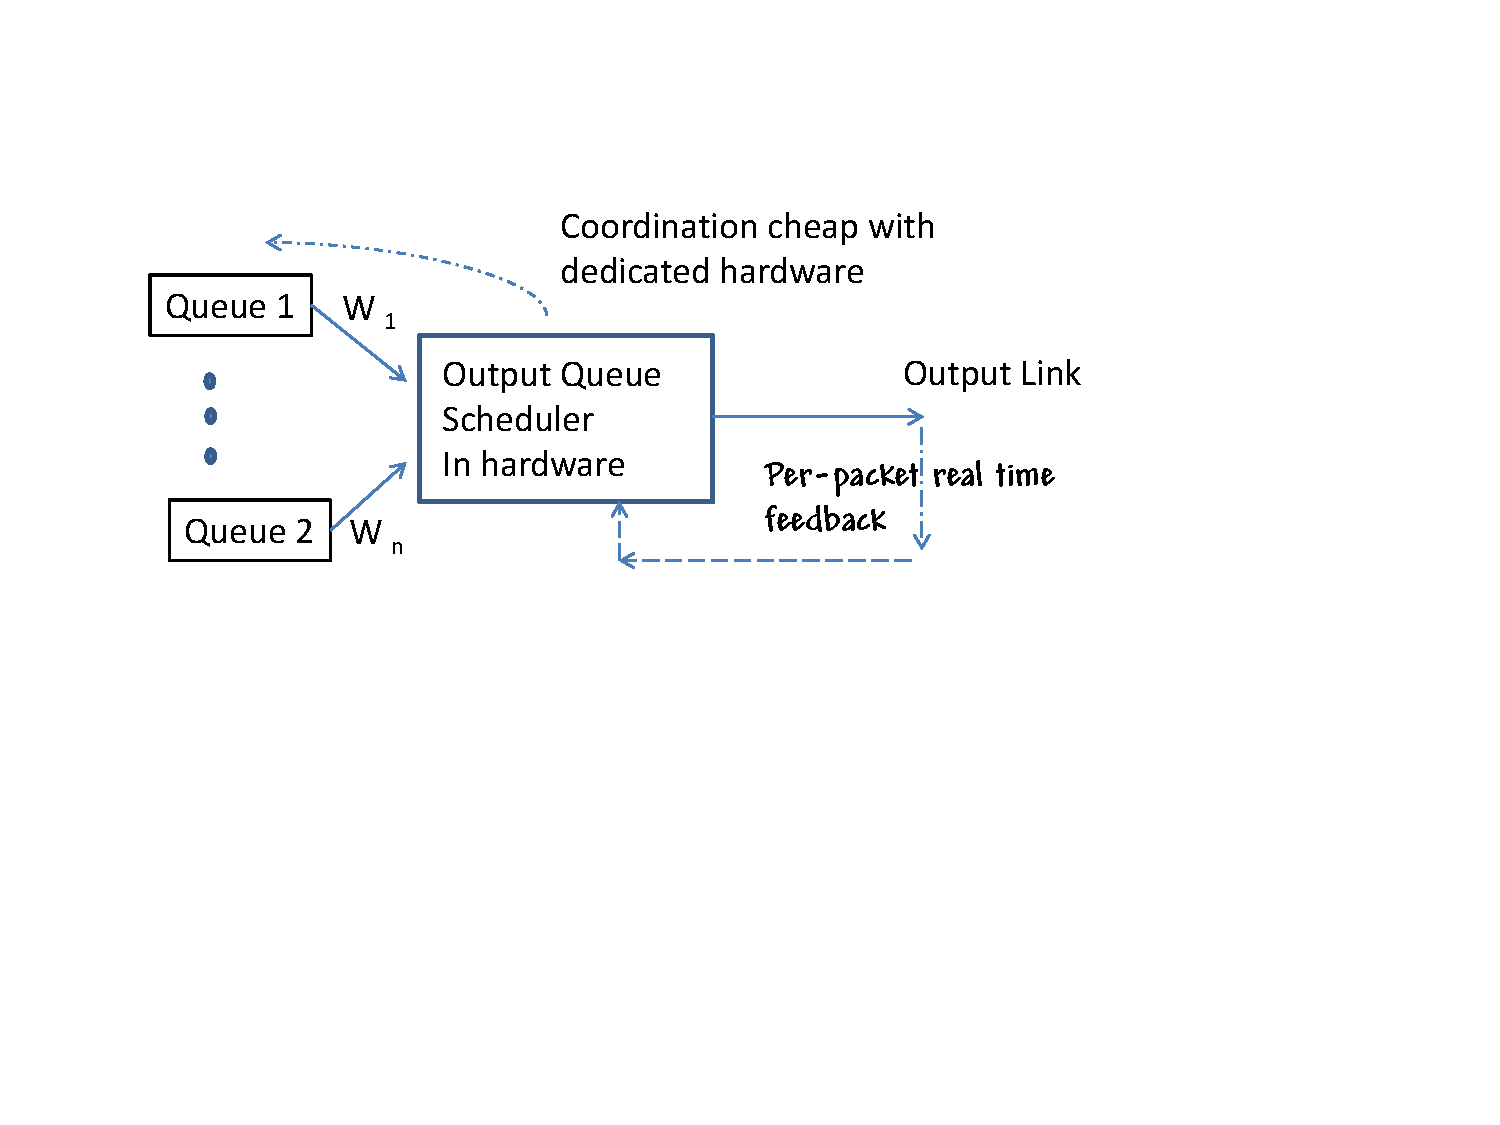
\includegraphics[width=0.3\textwidth,trim=6mm 90mm 20mm 10mm]{figures/standardqosmodel}
\label{fig:qosmodel}
}
\subfigure[VM Fair Queuing model]
{
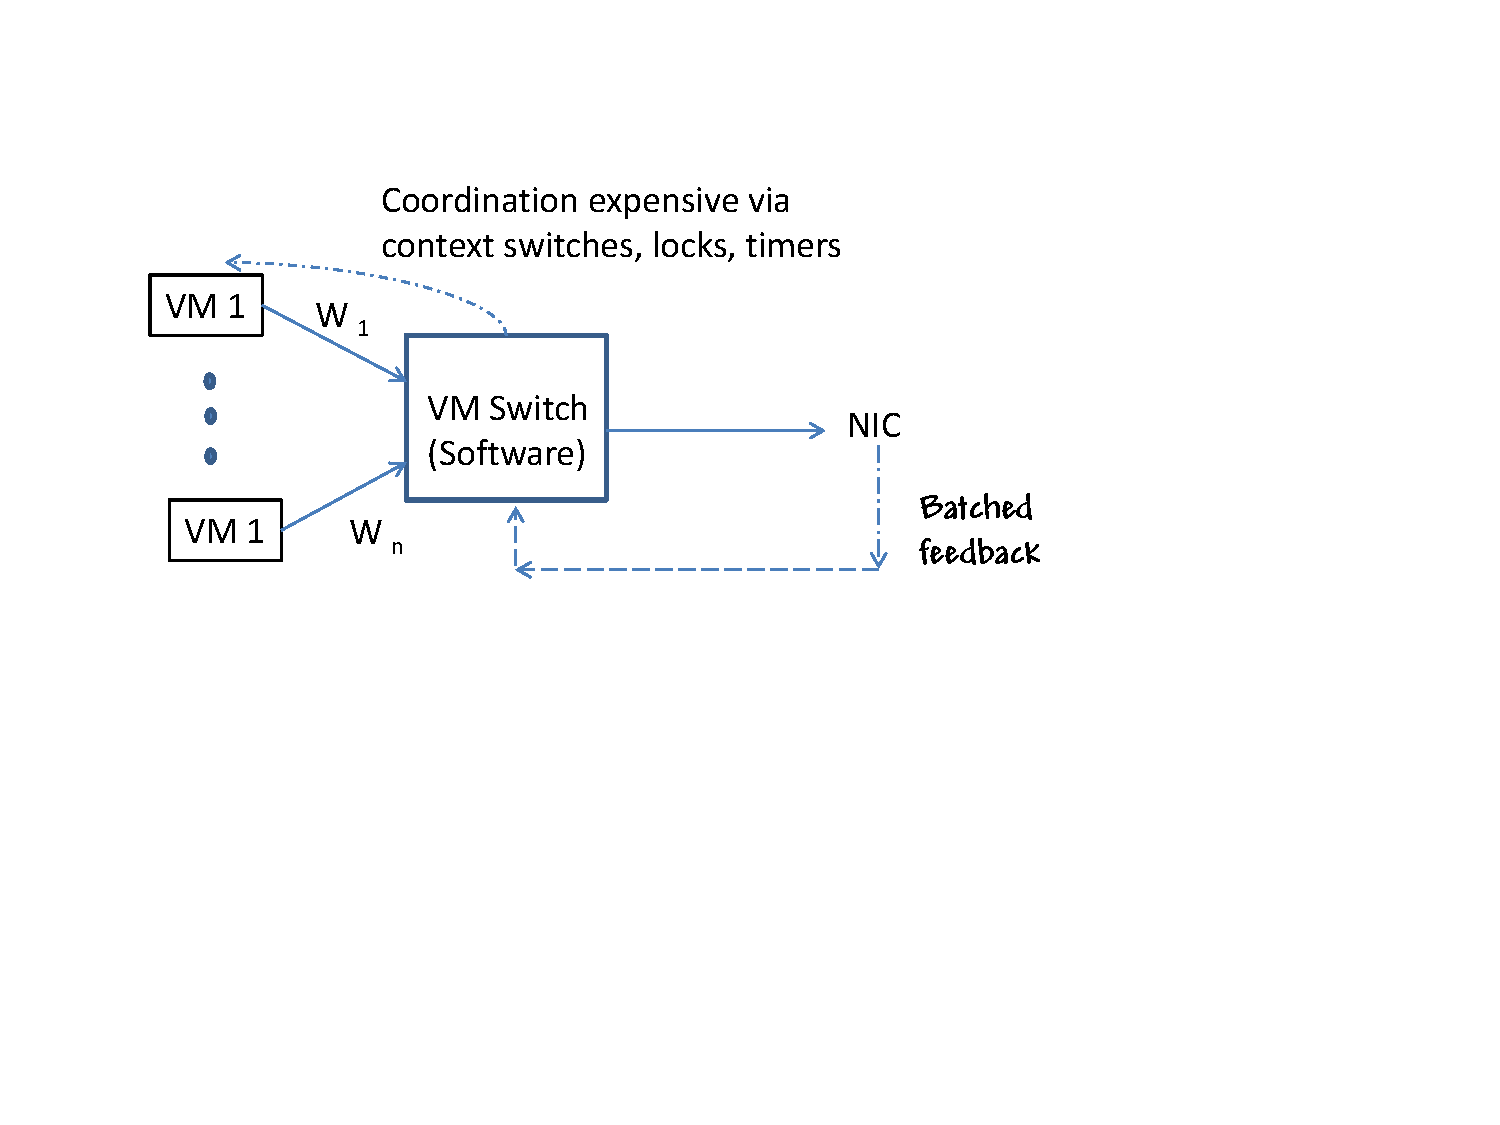
\includegraphics[width=0.3\textwidth, trim=6mm 90mm 20mm 10mm]{figures/vmqosmodel}
\label{fig:vmqosmodel}
}
\subfigure[Macro-Micro scheduler model]
{
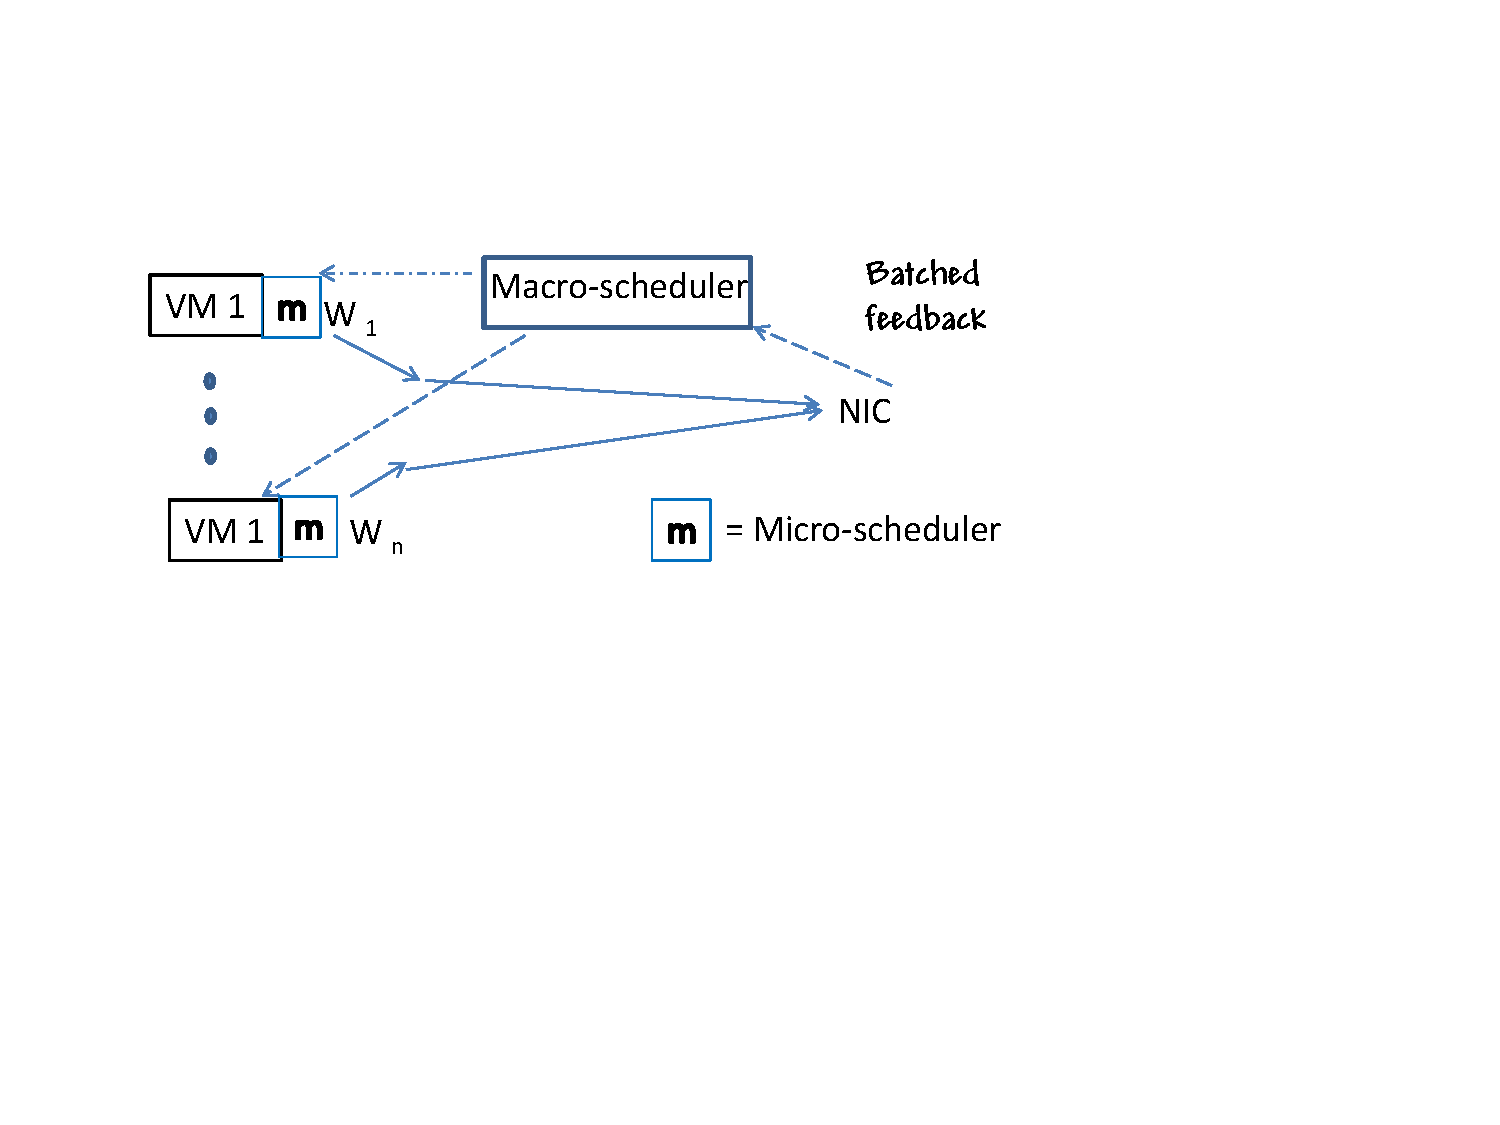
\includegraphics[width=0.3\textwidth, trim=6mm 90mm 20mm 10mm]{figures/macroschedule}
\label{fig:macroscheduler}
}
\vspace{-0.2em}
\caption{Scheduling models}
\label{fig:sched_mod}
\vspace{-0.5em}
\end{figure*}

\begin{figure}
\centering
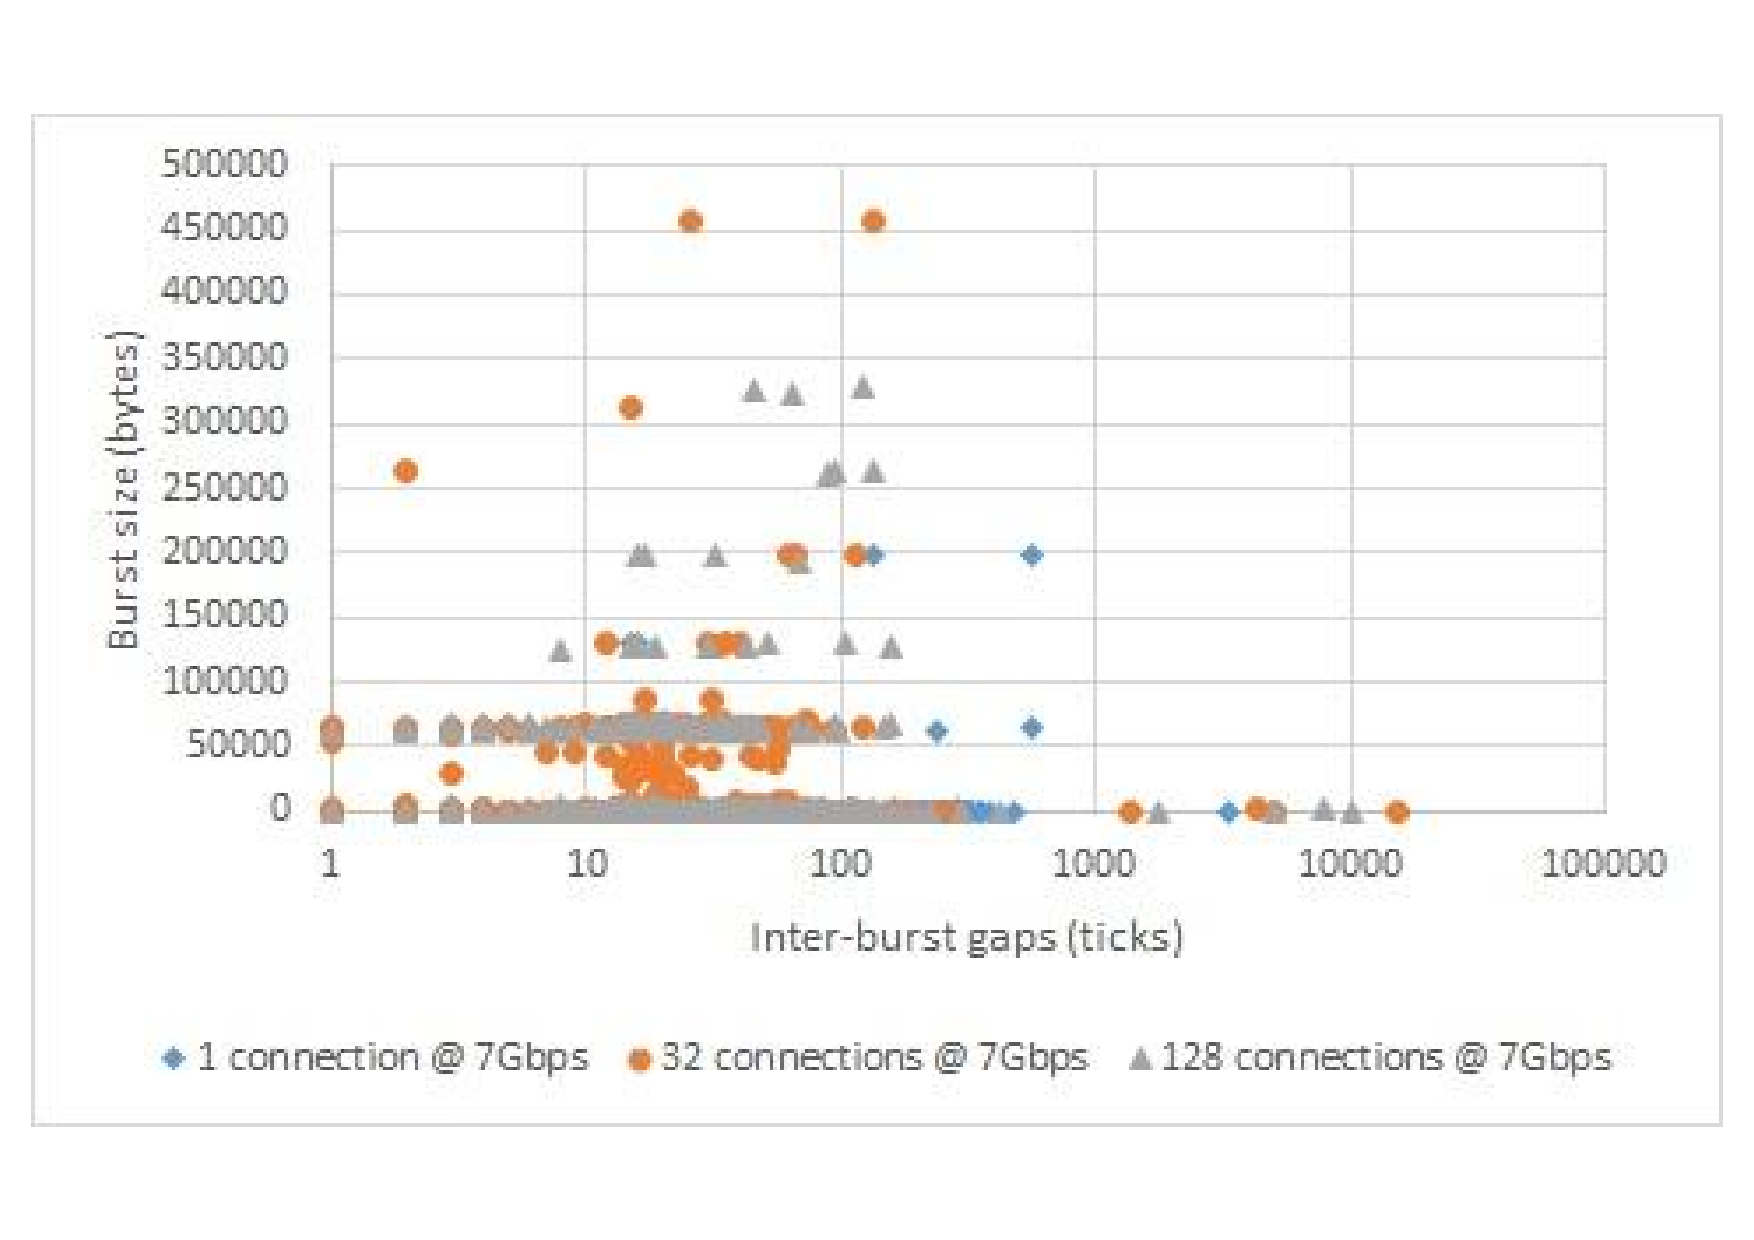
\includegraphics[width=0.7\columnwidth, trim=60pt 20mm 0pt 8mm]{figures/completesburst}
\caption{Burstiness of packet transmit-completes}
\label{completesburst}
\vspace{-3mm}
\end{figure}

Classical fair queuing model (Figure~\ref{fig:qosmodel}) used by algorithms such
as DRR~\cite{drr} and WF2Q~\cite{wf2q} make two implicit assumptions. First,
after packet transmission, the link alerts the hardware scheduler who chooses the
next packet to transmit. Second, the scheduler is able to keep up with link
speed.  Both assumptions are reasonable for hardware routers.

However, in our model  (Figure~\ref{fig:vmqosmodel}) the feedback loop between
link and scheduler is batched.  Modern NICs use mechanisms like Large Send
Offload (LSO) to minimize overhead, so they can only generate one send-complete
notification for a group of packets.  Without per-packet feedback, a DRR
software implementation will receive transmit completion notifications in
bursts. Figure~\ref{completesburst} shows the distribution of transmit-complete
notifications for a random 1000 contiguous samples, for three different traffic patterns.
The figure shows that the size of each notification can be on the order
of 500 kilobytes, and they can be microseconds (10000 ticks) apart. If
we run DRR under such conditions, it would cause transmit
jitters and packet drops, which, coupled with upper-layer throttling by the TCP
stack, will further exacerbate the issue.  Figure~\ref{completesburst} also shows that 
the distribution depends on the traffic pattern. Thus, the scheduler cannot
simply be tuned to respond to a certain distribution.

Implementations of weighted fair queuing algorithms like QFQ~\cite{qfq} solve
this problem by using technologies such as DPDK~\cite{dpdk} or
NetMap~\cite{netmap}, that allow them to bypass the NIC batching.  This is not
feasible in our scenario. For fine-grained scheduling, they also require more
CPU cycles than we can afford to spend.

We must also consider another subtle issue.  The software entity that
schedules packets from the queues must ensure that packets are en-queued to the
NIC's transmit buffer in the same order that they are de-queued from VSwitch
queues.  

There are two options to achieve this. First, the software could use a handle to
the NIC's transmit buffer.  This requires strong coordination between the
software module and the NIC's driver.  This is not desirable for a software
implementation on top of a hardware abstraction layer (e.g. NDIS in Windows), 
in a general-purpose OS that must work across many NIC vendors. A second
alternative is to make the software entity single-threaded so that each packet
is processed sequentially through the entire software stack from VSwitch to NIC
using a single processor. This is not scalable at multi-gigabit speeds.
Additionally, having to process packets on a single thread forces packets that
were processed on different processors to be then processed on a different
single processor, leading to cache misses which increase latency.  

Therefore,
our implementation needs to be able to schedule packets across multiple processors.  This
means we cannot satisfy the second implicit assumption that classical 
fair queuing models made (namely the scheduler can keep up with link speed) if the scheduler
 is invoked on a per-packet basis.  Signaling events across processors on a per-packet basis is prohibitively expensive.
For example, in Figure~\ref{completesburst}, transmission completes can occur on the order of
nanoseconds.  Signaling a scheduler at that granularity would require the CPU to spend
most of its time doing the signaling, leaving little cycles left for packet processing.  
It typically takes at least one dedicated core to saturate a 40Gbps link. 

Our solution is to divide the scheduler into two entities as shown in
Figure~\ref{fig:macroscheduler}.   The macroscheduler runs only every $T$
seconds and hence can run on a single thread.   The microschedulers, by
contrast, run on every packet based on tokens allocated by the microscheduler.   

While this model reduces overhead, it has obvious drawbacks because allocations
can only occur in units of $T$ seconds. Thus, our evaluation will focus on the
worst case time for a VM to ramp up to its guaranteed bandwidth, and it's
counterpart: the minimum amount of time needed to redistribute ``unused''
bandwidth from a VM that is not fully using its allocated bandwidth to other
active VMs. 

\section{MBFQ Algorithm}
\label{sec:algorithm}

\begin{figure}
\begin{algorithmic}
\State //
\State // MG: min guarantee (what the VM has paid for)
\State // SR: measured ssend rate since last macro scheduler iteration.
\State // TR: computed target rate for this iteration.
\State // AR: currently allocated rate
\State //
\State $residualBandwidth = lineRate$
\State $totalNeedsMoreWeight = 0$
\end{algorithmic}
\caption{}
\end{figure}

The main idea of MBFQ is to work in intervals of length $T$ where $T$ is
sufficiently large to reduce variance in measurement of sending rates for
typical network applications, and yet not too much larger than is strictly
necessary because the larger $T$ is, the larger $T_{inc}$ and $T_{dec}$ is.
This is because the macroscheduler only adjusts allocated rates in intervals of
length $T$.   We will show in the experimental section that if $T$ is around
$100$ msec, then the standard deviation is around $5\%$ for a TCP sender; while
the deviation goes down to $1\%$ as $T$ increases to $1$ seconds, it also slows
down responsiveness.  Hence our code uses $T = 100$ msec as a default.

The basic idea is simple.  We measure what every VM has sent in the last $T$
seconds and store in a variable $SR$ (for send rate).  In the first phase, by
comparing the sent rate to the amount  allocated to that VM in the last interval
($AR$), we make an estimate of whether this VM's allocation should (in an ideal
world with no constraints) increase or decrease and compute a target rate $TR$
in this ideal world. Then in a second phase, we incorporate the reality of a
fixed pot of link bandwidth and the other VMs that wish to send in order to
enforce fair-queuing and congestion freedom.

{\bf Phase 1: Determining Ideal Rates:}  First, we determine ideal rates for
each VM in an world where this VM is the only player based on past performance.
For example, if $SR > 0.95 AR$, then there is a case to be made that the VM
should be allocated more bandwidth (it has used what it was allocated).  Asking
a VM to use up everything it was allocated seems too strict, becausae of natural
variations in sending rates.  Of course, $95\%$ is merely a parameter.    

Similarly, if a VM's sending rate has fallen by some percentage of its allocated
rate, we might want to reduce the VM' s allocated rate.  Here we might choose to
be cautious.  A VM that has paid for $4$ Gbps. and was allocated that much, may
be measured to fall briefly below $4$ for a few intervals.  While if this
situation persists, we should reallocate the bandwidth, we wish to guard against
short term fluctuations that cause the algorithm to too eagerly reclaim
bandwidth.  Since it takes a few intervals to rise again, we choose to defend
against this by rising fairly quickly (say in 4 periods), but reclaiming
bandwidth at a much slower rate (say 10 periods).   

In summary, the first phase of the algorithm decides a target rate $TR$ based on
past sending performance.  If the VM has used its allocation, we mark it for
increase; otherwise, we keep it the same or even decrease it (after some number
of periods demonstrating this behavior) to close to its sending rate.    This
brings up the question: how should we increase a VM (still in an ideal world, we
will consider sharing in the second phase).  

To see the difficulty, suppose a VM $A$ has paid $2000$ a month for $5$ Gbps of
traffic and has been idle for a long time, and hence was allocated only a small
minimal amount of bandwidth of say $10$ Mbps.  Other VMs are using portions of
$A$'s bandwidth.  $A$ now decides to initiate a large data transfer which
requires its full guaranteed rate.   But $A$ has been allocated only $10$ Mbps.
We wish $A$ to rise rapidly from $10$ Mbps to $5$ Gbps.

In the first interval after $A$ initiates the data transfer $A$ will be measured
to have sent $10$ Mbs.  Since $A$ has shown intent to send, why not increase $A$
directly to $5$ Gbps.   The difficulty is if $A$ for other reasons can only send
at say $1$ Gbps.  In that case raising $A$ to $5$ can "waste" 4 Gbps for one
interval.  So a more cautious strategy seems to be in order.

Instead, we keep some state and (almost like TCP) and gradually increase $A$'s
allocations, taking care to bound $A$'s rise to its guaranteed rate.   For
example, in our current code, in the first period, we give $A$, $20\%$ more
allocation; if $A$ uses that up, we give $A$, $50\%$ more bandwidth.  However,
after some number of periods in which $A$ uses up all its allocations, we simply
aim to give $A$ at least its guaranteed bandwidth.   We bound that by 4 periods
in our current code.    

{\bf Phase 2:  Preventing Congestion and Enforcing Fair Sharing:}  So far the
algorithm has only determined the ideal allocations for each VM based on their
traffic pattern displayed in the last period.   However, to achieve
congestion-freedom, statistical multiplexing and fair sharing we must do more.
If the sums of the ideal rates computed in the first phase exceeds the lnk
bandwidth, we must prevent congestion.  If some VMs's ideal rates are below
their guaranteed rates, we must distribute unused bandwidth in proportion to the
weights of all flows that wish to use this bandwidth.  

Phase 2 begins by initializing each VM's allocated rate to be the m:w
inimum of its
ideal rate and its guaranteed rates.  This initial allocation guarantees
congestion freedom since by definition, the sum of the guaranteed rates cannot
exceed the link bandwidth.  But it can leave bandwidth on the table. This
remaining bandwidth is the link bandwidth minus the sum of the initial
(conservative) allocations.

To distribute "remaining" bandwidth, the algorithm marks the VMs whose ideal
target rates are more than their guaranteed rates as VMs that "need more
bandwidth".  Phase 2 then goes through a loop where it allocates the remaining
bandwidth to the needy VMs in proportion to their weights.  

This is subtler than it may appear.   At the end of one sub-iteration of this
second allocation phase, one may have allocated a VM more than its ideal rate
calculated in the first phase.  Since, the ideal rate is our proxy for what the
VM would desire in an ideal world without sharing, we remove this bandwidth and
iterate again.  

Once again, we mark VMs whose allocated rates are still less than their ideal
rates as needy, and allocate the remaining bandwidth among the still needy VMs.
This iteration continues until no bandwidth is left or no VMs are needy.   We
can prove that this loop terminates in that at least one VM will be removed from
the needy list in each iteration.  Note that these iterations within Phase 2 are
merely a few lines of code that run in nanoseconds (not in intervals of $T$); so
even doing this for 100s of VMs will not take be too slow.

The initialization for the MBFQ algorithm is shown in
Figure~\ref{initialization}.  Note that $RUStage$ (for Ramp Up Stage) is a state
variable that tracks the number of iterations over which a VM has been
increasing.  Every time a VM comes close to it's target, this counter is
increased (but to no more than $3$); every time a VM falls significantly below
its target this counter is decreased.  The 

\subsection{PseudoCode}

The pseudocode for the first part of Phase 1 is shown in
Figure~\ref{phase1start}. This code determines the slope of the VM's bandwidth
change (needs to increase, decrease or stay the same) by comparing the amount
allocated in the last period to what the VM sent, using some percentage
thresholds for some margin.  If it is falling, $RUStage$ is decreased; if it is
increasing $RUStage$ is incremented, always being careful to keep $0 \leq
RUStage \leq 3$. 

The pseudocode for the second part of Phase 1 is shown in
Figure~\ref{phase1finish}.  This is where the number of consecutive iterations
over which a VM has been determined to increase (tracked by $RUStage$) is used
to determine how aggressive an ideal increase to allocate to the VM, starting
from a modest $10\%$ increase all the way to at least the guaranteed bandwidth
in 4 iterations.

The pseudocode for the first part of Phase 2 is shown in
Figure~\ref{phase2start}.  It uses a new variable called $TempRate$ that is
initialized to be no more than the guaranteed rate.   This is then used to
compute how much bandwidth is left over, and which VMs can (based on their ideal
allocations) use up this remaining bandwidth.

The pseudocode for the second part of Phase 2 is shown in
Figure~\ref{phase2finish}.   It is a loop that allocates the excess to all the
needy VMs. If each VM then remains below its ideal target rate, the loop
terminates.  However, if some VM is allocated more than it uses, this wasted
bandwidth is added back to the remaining bandwidth and the loop continues.



\section{Experimental Evaluation}
\label{sec:experiments}

We have evaluated MBFQ extensively. Due to lack of space, we only present
selected microbenchmarks in this paper. Our microbenchmarking testbed consists
of two Dell PowerEdge R410 servers.  Both servers have four 2.26GHz cores, with
hyper-threading enabled, which gives it 8 logical processors.  Each machine has
8GB of RAM and 10G NIC.  Both machines run a flavor of Windows Server OS with
Hyper-V enabled for network virtualization. This configuration emulates our
common use case: VMs communicating with other VMs in the same data
center.~\footnote{Most of the traffic in modern data centers is intra-DC
traffic~\cite{fb,cosmos}.} \fixme{invalid ref}

\subsection{Picking a Timer Period for Measurement}
{\bf Question:}  The macrosheduler runs every $T$ time units. What is the right
value of $T$?

{\bf Motivation:}  As discussed earlier, it can take up to three iterations (thus
$3*T$) for the macroscheduler to allocate a VM with its minimum
guaranteed bandwidth. Therefore, we don't want $T$ to be too large. On the other hand,
recall that we measure send rate over the same time period. If $T$ is too small,
the measured send rate of the VM ($SR$) may be inaccurate. The primary source of
inaccuracy is inherent burstiness of TCP. To estimate the inaccuracy for
various values of $T$, we carried out the following experiment.

{\bf Experiment}: A single VM hosted on one of the servers sends data to
an external server using TCP. In all, 32 TCP connections were used. The application 
generated data at 7.2Gbps. All rate
allocation functionality of MBFQ was disabled, only the measurement code was
active.  We logged the measured send rate ($SR$) over 100 intervals.  We
repeated experiment for values of $T$ ranging from 15ms to 1000ms.
Figure~\ref{variation} shows the standard deviation as a function of $T$.  

\begin{figure}
\centering
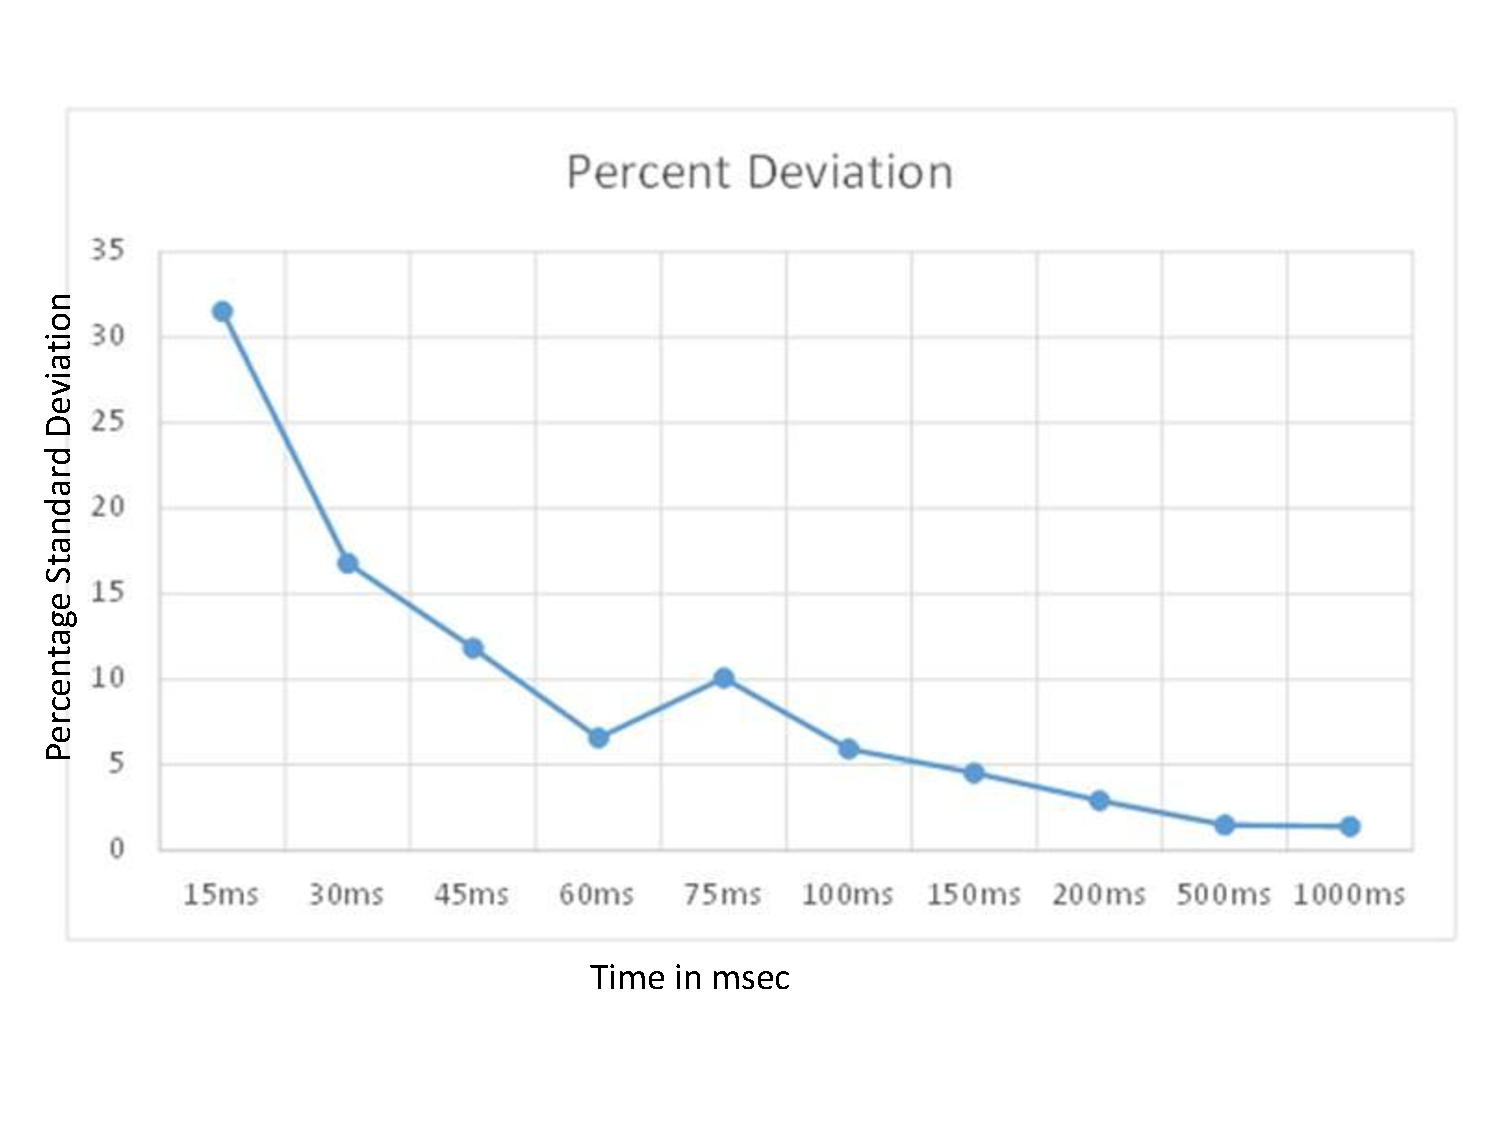
\includegraphics[width=0.7\columnwidth, trim=60pt 20mm 0pt 8mm]{figures/variation}
\caption{Impact of $T$ on variance in $SR$}
\label{variation}
\vspace{-3mm}
\end{figure}

{\bf Discussion:} A value of $T$ between 60 - 100ms reduces standard deviation
of $SR$ to $5\%$.  Larger $T$ will lead to further reduction, but decrease is
small.

\subsection{Bandwidth Ramp Up and Ramp Down}
\label{sec:fairshare}
{\bf Question:} A VM may have to wait for up to three macroscheduler intervals to reach its
minimum guaranteed bandwidth. Also, we wait for up to 500 milliseconds before we
reclaim bandwidth from a VM that is not fully using the allocated bandwidth. Are
these time intervals appropriate?

{\bf Motivation:}  While the allocated bandwidth to VM ramps up to the minimum
guaranteed bandwidth in three intervals, the VM may not be able to ramp up as
quickly, due to limitations of the TCP congestion control. Furthermore, waiting
for 500 milliseconds before reclaiming the bandwidth may lead to
under-utilization of the link.

{\bf Experiment:}  A test machine hosts 4 VMs with the following
minimum bandwidth guarantees: VM1: 100Mbps (relative weight: 1), VM2: 100Mbps
(relative weight: 1), VM3: 1Gbps (relative weight: 10), VM4: 3Gbps (relative
weight: 30). Each of the VMs sends traffic to an external machine ("client
machine") over the shared 10G external physical NIC.  The link is configured to
share 9.5Gbps among the VMs.  Each VM is always 
backlogged and tries to send data as fast as it can.

Figure~\ref{fairsharing}  shows the transmit bandwidth for each VM, and the
total transmit bandwidth in several phases. 

\begin{figure}[h]
\centering
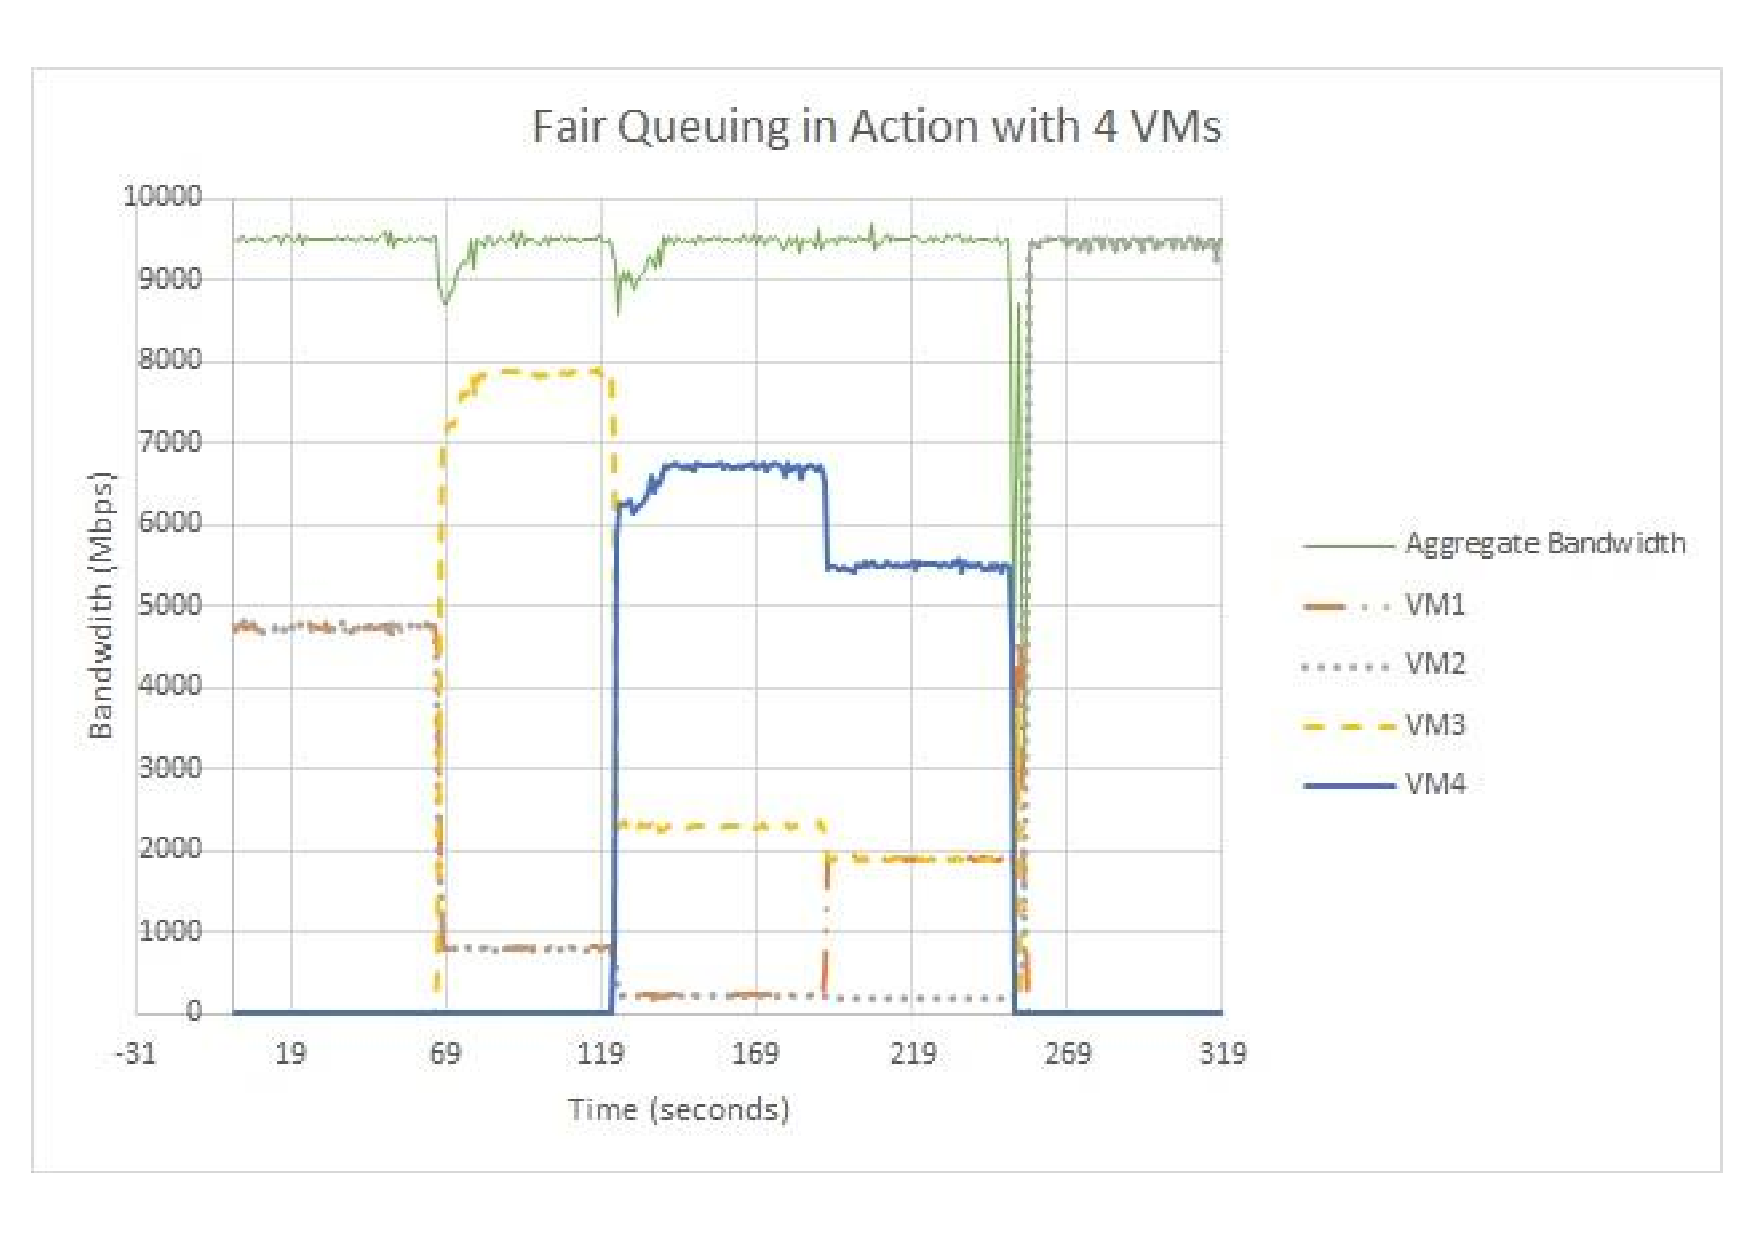
\includegraphics[width=0.8\columnwidth,trim=60pt 20mm 0pt 8mm]{figures/fairsharing}
\caption{Ramp up and ramp down test}
\label{fairsharing}
\vspace{-3mm}
\end{figure}

{\bf Phase 1:}  At time 0, only VM1 and VM2 are active. As expected, they share
the bandwidth equally, with each getting 4.75Gbps.

{\bf Phase 2:} At time 69, VM3 starts transmitting. MBFQ quickly
throttles VM1 and VM2 to 792Mbps each, while VM3 is allowed to use 7.92Gbps. 

{\bf  Phase 3:} At time 119, VM4 starts transmitting. The four VMs now
get their weighted fair share: VM1 and VM2 get 226Mbps, VM3
gets 2.26Gbps and VM4 gets 6.79Gbps. 

{\bf  Phase 4:} At time 189, we change the min bandwidth guarantee of VM1 from 100Mbps to
1Gbps. MBFQ allocation quickly converges to the expected rates: VM1 and VM3
now both transmit at the same rate, and the rates of VM2, VM3, and VM4 were reduced
to accommodate the increase in VM1's rate.

{\bf Phase 5:} At time 249, VM1, VM3, and VM4 stop sending. VM2 quickly
ramps up to consume the full link bandwidth.

{\bf Discussion:} We see that while MBFQ generally performs well, there are dips
in link utilization at times 69 and 119 as VMs ramp up. The dips in the aggregate
bandwidth at the beginning of phases 3
and 4 are due to our desire to allow a VM to quickly attain minimum
guaranteed bandwidth. As VM3 and VM4 are ramping up, the algorithm detects that
the VMs requests for additional bandwidth in several consecutive iterations.
Therefore, in order to quickly provide the VMs their subscribed bandwidth, after
three consecutive iterations of additional bandwidth requests, the algorithm
allocates the full fair share of bandwidth to the VM. However, even after
    the bandwidth is allocated, the VMs could take some time to consume all allocated
bandwidth, due to
TCP artifacts. Thus, the dip represents a trade-off between how fast the
algorithm should grant a VM its fair share versus how cautious it should be in
allocating the VM bandwidth that it might not be ready to consume (and thus risk
being non-work conserving). A more extreme dip is seen at the
beginning of phase 5, we shall discuss that in Section \ref{reclaimbw}.

\subsection{Can we ramp up any faster?}

{\bf Question:}  Is the ramp up delay shown in Figure~\ref{fairsharing} for VM4
at 69 seconds caused by our algorithm or it due to the VM itself (e.g., its TCP
behavior)?

{\bf Motivation:} The previous experiment suggests the algorithm may be too slow
in allocating bandwidth to a newly active VM.  

{\bf Experiment:} We measure bandwidth ramp up in two scenarios.  First, we
measure a  ``standalone'' scenario where VM3 is the only VM transmitting (i.e. the link
was idle before VM3 started sending).  Second, we measure a  ``sharing'' scenario
in which the link was fully utilized before VM3 started sending. When VM3 starts
sending, MBFQ performs bandwidth allocation to give VM3 its fair share.

\begin{figure}[h]
\centering
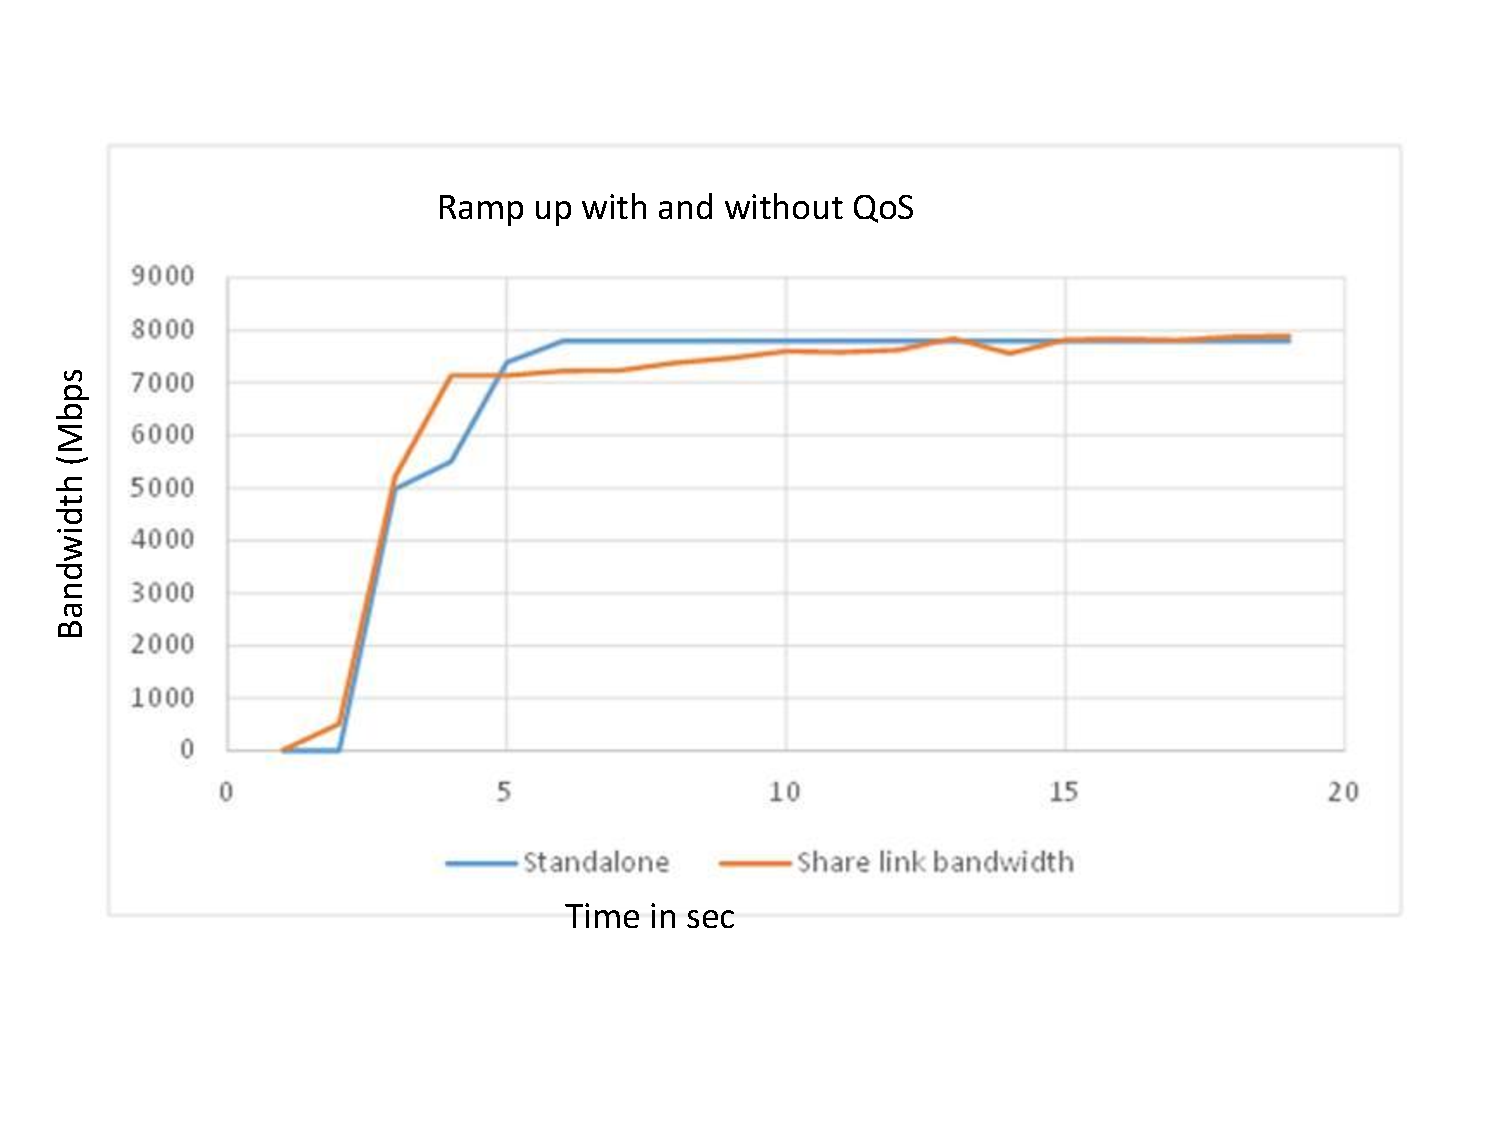
\includegraphics[width=0.7\columnwidth,trim=60pt 40mm 0pt 8mm]{figures/rampupcomparison}
\caption{TCP and MBFQ ramp up}
\label{rampupcomparison}
\vspace{-3mm}
\end{figure}

{\bf Discussion:} As seen in Figure~\ref{rampupcomparison}, it takes about the
same amount of time in both scenarios for VM3 to achieve most of its bandwidth
(up to 7Gbps). However, it takes an additional 15s for VM3 to reach its steady
state  in the "Share link bandwidth" scenario. However, in the sharing scenario,
the VM is transmitting on top of a NIC that is already fully utilized.
But in the standalone case, the VM is transmitting on top of an idle NIC. 

{\bf Conclusion:} It is probably not worthwhile 
to ramp up faster because TCP may not be able to fully utilize the extra
bandwidth quickly.

\subsection{How fast should we reclaim bandwidth?}
\label{reclaimbw}
{\bf Question:}  The faster we reclaim bandwidth the
faster we redistribute it other needy VMs who can use it. How large should the
reclaim period $T$ be?

{\bf Motivation:} 
We see a large dip in the utilization at the beginning of Phase 5 in
Figure~\ref{fairsharing} when VM1, VM3, VM4 stop sending.  In addition to the
TCP ramp-up time of VM2, the dip is also partly due to another parameter in the
algorithm where we configure the algorithm to wait for 500 milliseconds before
reclaiming residual bandwidth.  Unfortunately, this is a tradeoff.  The faster we
reclaim, the more likely the algorithm is to spuriously reclaim bandwidth from a
paid customer VM which has short term bursts.

{\bf Experiment:} We measure the impact of different reclaim timer values on the
throughput of a large file transfer operation in a VM.  We have VM1 host a large
file that is being copied to a remote machine, while VM2, VM3, VM4 send background CBR traffic
to fill up the idle link.  The file transfer application on
VM1 uses about 800Mbps, and the rest of the link bandwidth is distributed among
VM2, VM3, VM4.  We change the wait time parameter from No Wait (at every
macroshedular iteration, bandwidth is immediately reclaimed if VM1 is
sending less than 85\% of its allocated rate) to 1000ms wait (bandwidth is not
reclaimed unless the VM has been sending less than 85\% of its allocated rate in
the last 1000ms)

\begin{figure}[h]
\centering
\subfigure[Reclaim timer of 500 msec and 1000 msec]
{
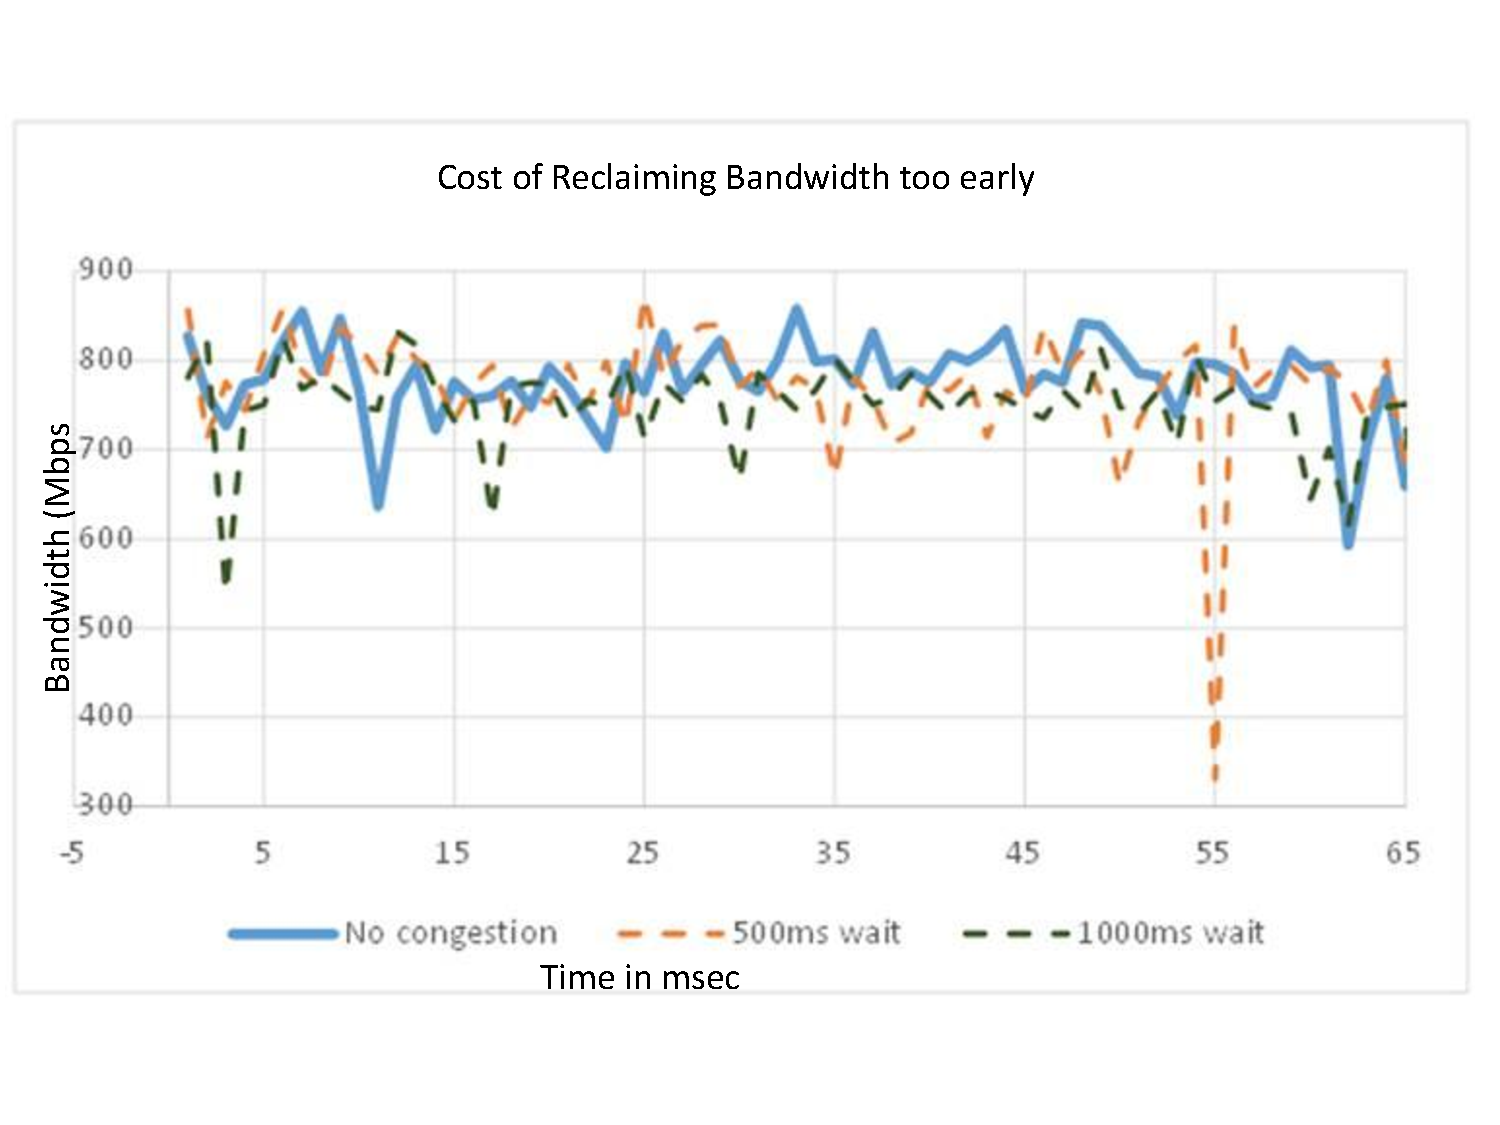
\includegraphics[width=0.7\columnwidth,trim=60pt 20mm 0pt 8mm]{figures/rampdowntime1}
\label{rampdowntime1}
}
\subfigure[Reclaim timer of 0 msec and 200 msec.]
{
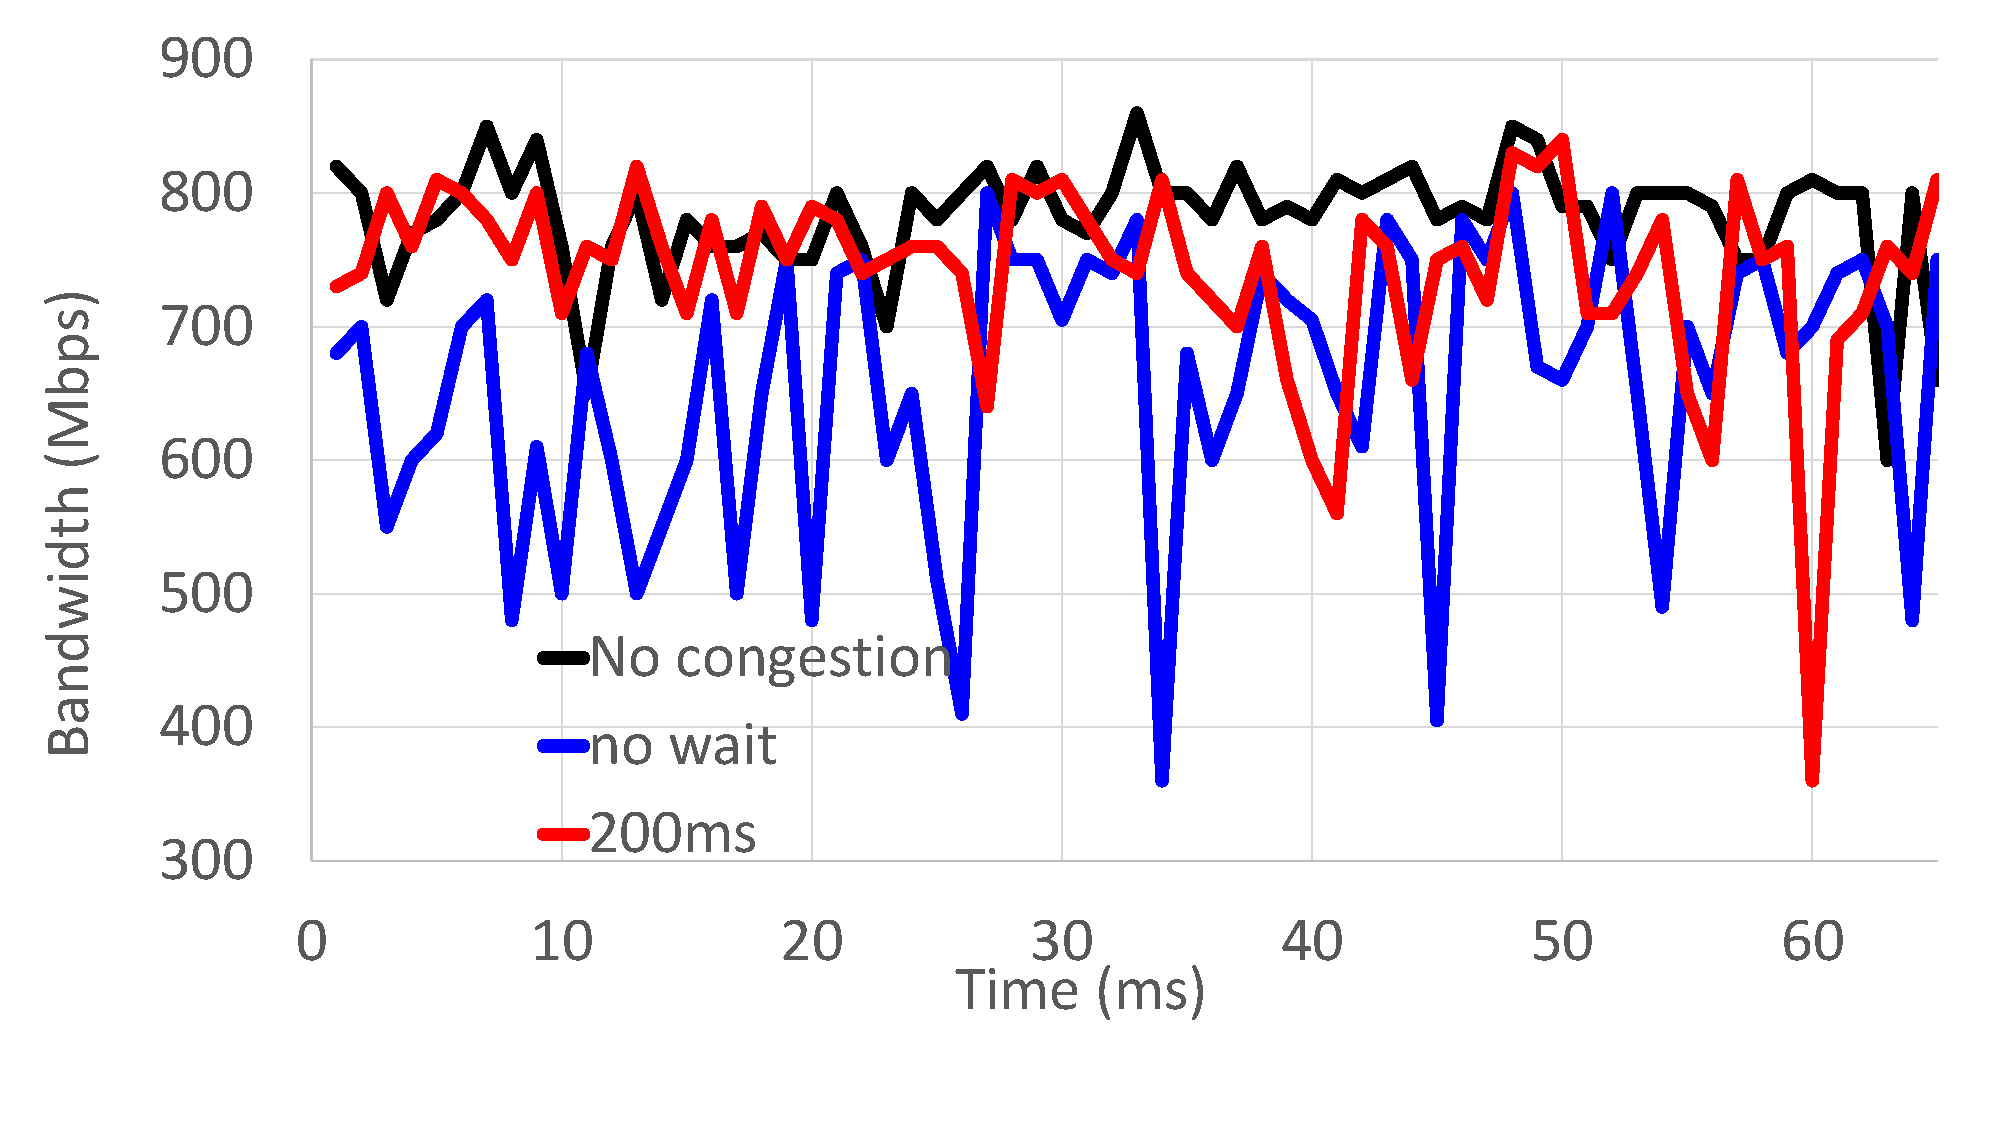
\includegraphics[width=0.7\columnwidth,trim=60pt 20mm 0pt 8mm]{figures/rampdowntime2}
\label{rampdowntime2}
}
\vspace{-1em}
\caption{Impact of reclaim timer}
\vspace{-1em}
\label{fig:reclaim}
\end{figure}

Figure~\ref{rampdowntime1} shows that the bandwidth stays roughly the same with
MBFQ and without MBFQ with a reclaim timer of 500 msec (in fact 1000 msec looks
even worse, but that could be an artifact).   On the other
hand,Figure~\ref{rampdowntime2} shows that with instantaneous reclaiming
(reclaim timer of 0) the bandwidth allocated to the VM is significantly affected
(by around 50\%) and its noticeable even at a reclaim timer of 200 msec.

{\bf Conclusion:}  A reclaim timer of around 500 milliseconds seems like a good
compromise. 

\bibliographystyle{abbrv}
\bibliography{qos}

\end{document}
